\documentclass[tikz,border=5mm]{standalone}
\usetikzlibrary{decorations.markings}

\begin{document}
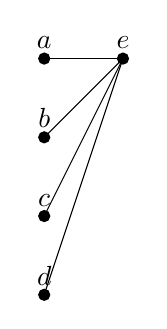
\begin{tikzpicture}[every loop/.style={min distance=30mm}]

    % these are the vertices
    \draw[fill=black] (5,5) circle (2pt) node[above] {$a$};
    \draw[fill=black] (5,4) circle (2pt) node[above] {$b$};
    \draw[fill=black] (5,3) circle (2pt) node[above] {$c$};
    \draw[fill=black] (5,2) circle (2pt) node[above] {$d$};
    \draw[fill=black] (6,5) circle (2pt) node[above] {$e$};

    \draw (5, 5)-- (6, 5);
    \draw (5, 4)-- (6, 5);
    \draw (5, 3)-- (6, 5);
    \draw (5, 2)-- (6, 5);

\end{tikzpicture}
\end{document}
